\documentclass{../../slides-style}

\slidetitle{Практика, архиватор Хаффмана}{02.11.2022}

\begin{document}

    \begin{frame}[plain]
        \titlepage
    \end{frame}

    \begin{frame}
        \frametitle{Напоминание идеи алгоритма}
        \begin{columns}
            \begin{column}{0.5\textwidth}
                \begin{itemize}
                    \item Считаем частоты символов во входной строке
                    \item Склеиваем два самых редких в один псевдосимвол, пока не получили одно дерево
                    \item Строим по дереву префиксный код в виде таблицы
                    \item Бежим по строке, заменяя символ на его код
                    \begin{itemize}
                        \item Используем битовый буфер для формирования байта выдачи
                    \end{itemize}
                    \item При разархивировании бежим от корня до листа
                \end{itemize}
            \end{column}
            \begin{column}{0.5\textwidth}
                \begin{figure}[htp]
                    \centering
                    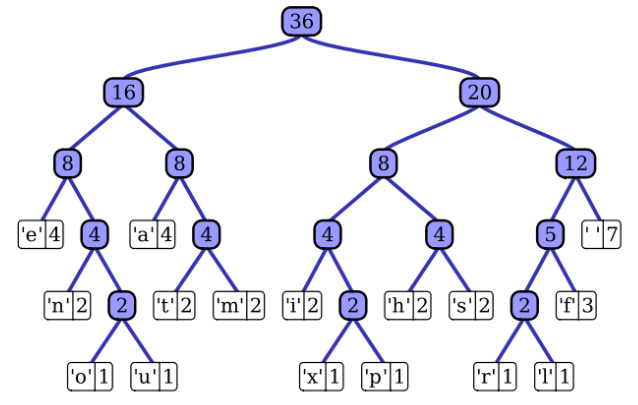
\includegraphics[width=0.8\textwidth]{huffman-tree.png}
                    Пример: ``this is an example of a huffman tree''
                \end{figure}
            \end{column}
        \end{columns}
    \end{frame}

    \begin{frame}
        \frametitle{Задача}
        \begin{enumerate}
            \item Описать двоичное дерево, хранящее символы и частоты, в отдельном модуле
            \item Построить дерево частот
            \item Построить таблицу с префиксными кодами
            \item (*) Получить сжатую строку
            \item (*) Оценить степень сжатия
            \item (*) Реализовать разжатие
        \end{enumerate}
    \end{frame}

\end{document}